\chapter{Ensayos y mediciones}

\section{Medición de ripple (sin regulador)}

Para poder realizar las siguiente mediciones en este primer ensayo, previamente se realizo en la placa la soldadura del puente diodo y el filtro.

\subsection{En el filtro capacitivo y determinación de parámetros.}

Se tomaran medidas de la tension tanto en el punto bajo como en el punto alto del transformador variando la
corriente desde el vacio (0 A) hasta llegar a plena carga (1,5 A). Con las mediciones vamos a poder calcular los siguientes tres factores:
Regulacion de voltaje, resistencia variable y factor de ripple.\\

\subsubsection{Punto bajo}

\begin{table}[H]
  \centering
  \begin{tabular}{|c|c|}
    \hline
    $V_{vacio}$ & 17,71 V \\ \hline
    $V_{0,5 A}$ & 15,80 V \\ \hline
    $V_{0,75 A}$ & 15,27 V \\ \hline    
    $V_{1 A}$ & 14,63 V \\ \hline
    $V_{1,25 A}$ & 14,10 V \\ \hline
    $V_{PlenaCarga}$ & 13,69 V \\ \hline
  \end{tabular}
  \caption{Mediciones en el punto bajo}
\end{table}


\begin{figure}[H]
  \centering
  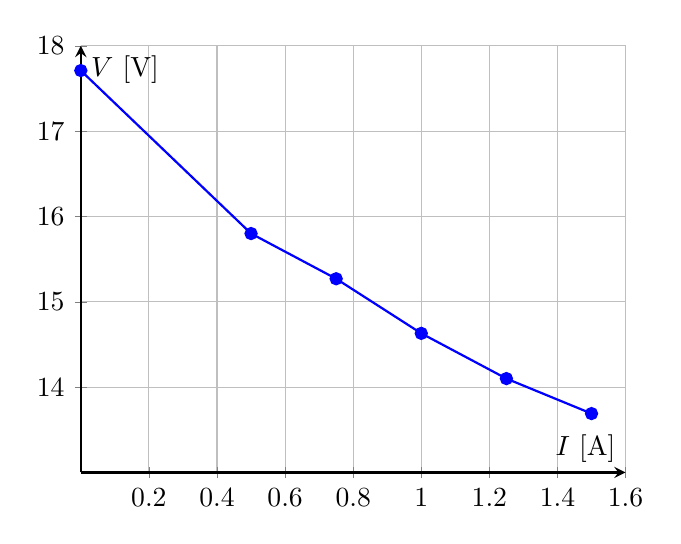
\begin{tikzpicture}
    \begin{axis}[
      axis lines = middle,
      xlabel = {$I$ [A]},
      ylabel = {$V$ [V]},
      domain = 0:1.5,
      samples = 200,
      grid = both,
      width=8.5cm,
      height=7cm,
      xmin = 0, xmax= 1.6,
      ymin = 13, ymax = 18,
      thick
      ]
      \addplot[blue, mark=*] coordinates {
            (0, 17.71)
            (0.5, 15.80)
            (0.75, 15.27)
            (1, 14.63)
            (1.25, 14.10)
            (1.5, 13.69)
      };
    \end{axis}
  \end{tikzpicture}
  \caption{Vout vs Iout punto bajo}
\end{figure}

\subsubsection{Punto alto}

\begin{table}[H]
  \centering
  \begin{tabular}{|c|c|}
    \hline
    $V_{vacio}$ & 36,86 V \\ \hline
    $V_{0,5 A}$ & 31,89 V \\ \hline
    $V_{0,75 A}$ & 31,05 V \\ \hline    
    $V_{1 A}$ & 29,83 V \\ \hline
    $V_{1,25 A}$ & 28,55 V \\ \hline
    $V_{PlenaCarga}$ & 27,47 V \\ \hline
  \end{tabular}
  \caption{Mediciones en el punto alto}
\end{table}

\begin{figure}[H]
  \centering
  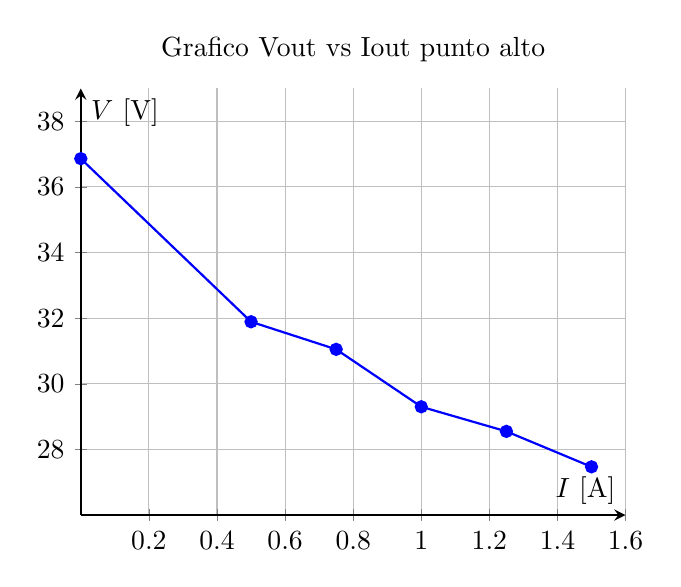
\begin{tikzpicture}
    \begin{axis}[
      axis lines = middle,
      xlabel = {$I$ [A]},
      ylabel = {$V$ [V]},
      domain = 0:1.5,
      samples = 200,
      grid = both,
      width=8.5cm,
      height=7cm,
      title = {Grafico Vout vs Iout punto alto},
      xmin = 0, xmax= 1.6,
      ymin = 26, ymax = 39,
      thick
      ]
      \addplot[blue, mark=*] coordinates {
            (0, 36.86)
            (0.5, 31.89)
            (0.75, 31.05)
            (1, 29.3)
            (1.25, 28.55)
            (1.5, 27.47)
      };
    \end{axis}
  \end{tikzpicture}
\end{figure}

\subsection{Determinación de resistencia interna del transformador más la de los diodos.}

\subsubsection{Punto bajo}

Para calcular la regulacion de voltaje se utiliza la siguiente formula:

\begin{equation}
  \begin{aligned}
    RV &= \dfrac{V_{vacio} - V_{PlenaCarga}}{V_{PlenaCarga}} 100\percent \\
    RV &= \dfrac{17,71\V - 13,69\V}{13,69\V} 100\percent = 29,36\percent
  \end{aligned}
\end{equation}

La resistencia interna esta dada por:

\begin{equation}
  \begin{aligned}
    R_{int} &= \dfrac{V_{PlenaCarga} - V_{vacio}}{-I_{carga}}\\
    R_{int} &= \dfrac{13,69\V - 17,71\V}{-1,5\A} = 2,68\ohm
  \end{aligned}
\end{equation}

Ahora mediremos el voltaje del ripple tanto con multimetro true RMS, como en el osciloscopio:

\begin{equation}
  V_{RippleMultimetro} = 908 mV
\end{equation}
\begin{equation}
  V_{RippleOsciloscopio} = 972 mV
\end{equation}
\begin{equation}
  V_{PicoaPico} = 2,75 V
\end{equation}

Factor de ripple:

\begin{equation}
  \begin{aligned}
    F_R &= \dfrac{V_{eficaz}}{V_{PlenaCarga}} 100\percent\\
    F_R &= \dfrac{908 mV}{13,69 V} 100\percent\\
    F_R &= 6,6325\percent
  \end{aligned}
\end{equation}

\subsubsection{Punto alto}
Para el punto alto repetiremos las formulas del punto bajo cambiando por los valores correspondientes: \\

Regulacion de voltaje:

\begin{equation}
  RV = \dfrac{36,68\V - 27,43\V}{27,43\A} 100\percent = 33,72\percent
\end{equation}

Resistencia interna:

\begin{equation}
  R_{int} = \dfrac{27,43\V - 36,68\V}{-1,5\A} = 6,16\ohm
\end{equation}

Ripple:

\begin{equation}
  V_{RippleMultimetro} = 0,83 V
\end{equation}

\begin{equation}
  V_{RippleOsciloscopio} = 0,88 V
\end{equation}

\begin{equation}
  V_{PicoaPico} = 2,5 V
\end{equation}

Factor de rippple:

\begin{equation}
  \begin{aligned}
    F_R &= \dfrac{0,83 V}{27,43 V} 100\percent\\
    F_R &= 3,0258
  \end{aligned}
\end{equation}


\section{Mediciones finales (con regulador)}

A continuación, se llevarán a cabo una serie de mediciones destinadas a verificar el correcto funcionamiento del regulador LM317 en la
fuente montada. Estas pruebas incluyen la medición de caída de tensión y corriente para alcanzar su potencia máxima, análisis de la
regulación de voltaje tanto en vacío como a plena carga, evaluación del ripple mediante osciloscopio y cálculo de su factor, así como la
medición de temperatura en el encapsulado del regulador para estimar su temperatura interna. Estas mediciones permitirán validar el
desempeño eléctrico y térmico del circuito en condiciones reales de operación.

\begin{figure}[h]
  \centering
  \includegraphics[width=0.70\textwidth]{images/placaMontada.png}
\end{figure}

\subsection{Regulación de voltaje.}

\begin{table}[H]
  \centering
  \begin{tabular}{|c|c|}
    \hline
    $V_{vacio}$ & 16,92 V \\ \hline
    $V_{PlenaCarga}$ & 16,29 V \\ \hline
  \end{tabular}
\end{table}

\begin{equation}
  \begin{aligned}
    RV &= \dfrac{16,92 - 16,29}{16,29} 100\percent\\
    RV &= 3,867
  \end{aligned}
\end{equation}

\subsection{Factor de ripple.}

\begin{equation}
  V_{RippleEficaz} = 353,55 . 10^{-6} V = 353,5 uV 
\end{equation}

\begin{equation}
  \begin{aligned}
    F_R &= \dfrac{353,5 uV}{16,29 V} 100\percent\\
    F_R &= 2,1703 . 10^{-3}\percent
  \end{aligned}
\end{equation}

\begin{figure}[H]
  \centering
  \includegraphics[width=0.70\textwidth]{images/medicionRipple.png}
  \caption{Visualizacion de riple en osciloscopio}
\end{figure}


\subsection{Cálculo de temperatura de juntura.}

\begin{figure}[H]
  \centering
  \includegraphics[width=0.95\textwidth]{images/calculoTemperatura.png}
  \caption{Calculo de la temperatura}
\end{figure}

\begin{equation}
  \begin{aligned}
    T_J - T_C = \theta_{JC} \times P_D \quad \Rightarrow \quad T_J = \theta_{JC} \times P_D + T_C
   \end{aligned}
\end{equation}

\[
  T_J \text{: Temperatura de la juntura interna}
\]
\[
  T_C \text{: Temperatura que mediremos del regulador}
\]
\[
  \theta_{JC} \text{: Resistencia termica de la juntura}
\]

Medimos la temperatura del regulador y usamos el dato de la resistencia termica de la juntura. \\

\begin{equation}
  \begin{aligned}
    \theta_{jc} = 5\dfrac{\circ C}{W}
  \end{aligned}
\end{equation}
\begin{equation}
  \begin{aligned}
    T_C = 60 \circ C
  \end{aligned}
\end{equation}

Entonces podemos calcular. \\

\begin{equation}
  \begin{aligned}
    T_J = (5\dfrac{\circ C}{W} . 15,19 W) + 60 \circ C
  \end{aligned}
\end{equation}

\begin{equation}
  \begin{aligned}
    T_J = 135,95 \circ C
  \end{aligned}
\end{equation}

   
\begin{figure}[H]
  \centering
  \includegraphics[width=0.70\textwidth]{images/medicionTemperatura.png}
  \caption{Medicion de la tempera en LM317}
\end{figure}

